\documentclass{nature3}
\usepackage{graphicx}
\usepackage{float}
\usepackage{verbatim}
\usepackage{hyperref}
\usepackage{amsmath}
\usepackage{amssymb}
\usepackage{aas_macros_nature}
\usepackage{lineno}

\linespread{1.0}
\linenumbers % turn line numbering on or off

\newcommand{\starname}{TIC 141146667}

\newcommand{\farcm}{\mbox{\ensuremath{.\mkern-4mu^\prime}}}%    % fractional arcminute symbol: 0.'0
\newcommand{\farcs}{\mbox{\ensuremath{.\!\!^{\prime\prime}}}}%  % fractional arcsecond symbol: 0.''0

\newcommand{\kms}{\ensuremath{\rm km\,s^{-1}}}
\newcommand{\ms}{\ensuremath{\rm m\,s^{-1}}}

\renewcommand*{\thefootnote}{\fnsymbol{footnote}}

%%%%%%%%%%%%%%%%
% INSTITUTIONS %
%%%%%%%%%%%%%%%%
\newcommand{\carnegie}{Observatories of the Carnegie Institution for Science, Pasadena, CA 91101, USA}
%%%%%%%%%%%%%%%%

%%%%%%%%%%
% VALUES %
%%%%%%%%%%
% NOTE: might need to be ingested before submission 
\newcommand{\stteff}{YYYY}
\newcommand{\stagemyr}{40}
\newcommand{\periodhr}{3.930}


%%%%%%%%%%%%%%%%%%%%%%%%%%%%%%%%%%%%%%%%%%
%%%%%%%%%%%%%%%%%%%%%%%%%%%%%%%%%%%%%%%%%%

\title{A Plasma Torus Around a Young Low-Mass Star}

\begin{document}

\author{Luke G. Bouma$^{1,2}$}

\maketitle

\scriptsize
\begin{affiliations}
\item \carnegie
\item Carnegie Fellow
\end{affiliations}
\normalsize

%%%%%%%%%%%%%%%%%%%%%%%%%%%%%%%%%%%%%%%%%%%%%%%%%%%%%%%%%%%%%%%%%%%%%%%%%%%%%%%
%%%%%%%%%%%%%%%%%%%%%%%%%%%%%%%%%%%%%%%%%%%%%%%%%%%%%%%%%%%%%%%%%%%%%%%%%%%%%%%

\begin{abstract}
\normalfont
% v1: removed a sentence for wordcount.  v0 is under abstract_title.txt
Approximately one percent of red dwarfs younger than 100 million years
show structured, periodic optical light curves suggestive of
transiting clumps of opaque material corotating with the star
\cite{Rebull2016,Stauffer2017,Rebull2018,Bouma2024}.  The
composition, origin, and even the existence of this material are
uncertain. The main alternative hypothesis is that these complex
periodic variables (CPVs) are explained by complex distributions of
dark starspots or bright faculae distributed across the stellar surfaces
\cite{Koen2021}.  Here, we present time-series spectroscopy and
photometry of a young ($t$=16\,Myr), rapidly-rotating
($P$=3.9\,hr) CPV, TIC~141146667. The spectra show coherent
sinusoidal Balmer emission at up to four times the star's equatorial
velocity, demonstrating the presence of extended clumps of
circumstellar plasma --- a plasma torus.  Given that long-lived
condensations of cool ($10^4$ K) plasma can persist in the hot
($10^6$ K) coronae of stars with a wide range of masses
\cite{CollierCameron1989,Townsend2005,Dunstone2006,Petit2013,Waugh2022,Daley-Yates2024},
these data support the idea that such condensations can become
optically thick around the lowest-mass stars, although the exact
source of opacity remains unclear.
\end{abstract}

\maketitle

%%%%%%%%%%%%%%%%%%%%%%%%%%%%%%%%%%%%%%%%%%%%%%%%%%%%%%%%%%%%%%%%%%%%%%%%%%%%%%%
%%%%%%%%%%%%%%%%%%%%%%%%%%%%%%%%%%%%%%%%%%%%%%%%%%%%%%%%%%%%%%%%%%%%%%%%%%%%%%%

% Main text – up to 3,000 words, excluding abstract, Methods,
% references and figure legends.

\section{Main}
\label{sec:main}

%\subsection{Introduction}
M dwarfs, stars with masses below about half that of the Sun, are the
only type of star to offer near-term prospects for detecting the
atmospheres of rocky exoplanets with water on their surfaces
\cite{NAP26141}.  Investment with JWST has proceeded accordingly.  How
an M dwarf's evolution influences its planets---especially the
retention of their atmospheres--- has concurrently become a major
theme in exoplanet and stellar astrophysics.  Previous work has
established that most M dwarfs host close-in planets
\cite{Dressing2015} that are often subject to long
circumstellar disk lifetimes \cite{Ribas2015}, to large doses of UV
radiation \cite{France2013}, and to a high incidence of flares and
coronal mass ejections \cite{Gunther2020}.  Nevertheless, despite excellent
work in these areas, the properties of the circumstellar plasma and
magnetospheric environments that bathe young, close-in exoplanets have
remained challenging to quantify.

One glaring example of our current ignorance is the complex periodic
variables (CPVs).  Figure~\ref{fig:lc} highlights the main object of
interest in this article, but over one hundred analogous objects have
now been found by K2 and TESS 
\cite{Rebull2016,Stauffer2017,Rebull2018,Zhan2019,Rebull2020,Bouma2024}.
These CPVs are
defined by their highly structured and periodic optical light curves, 
and most are M dwarfs with rotation periods shorter than two days.
Within current sensitivity limits, none have primordial disks
\cite{Stauffer2017,Bouma2024}.
However, $\approx$3\% of stars a few million years old show this
behavior, and the observed fraction decreases to $\approx$0.3\%
by $\approx$150\,Myr \cite{Rebull2020}.

The two leading hypotheses to explain the CPVs are either that
transiting clumps of circumstellar material corotate with the star
\cite{Stauffer2017,Gunther2022,Bouma2024}, or that these stars
represent an extreme in naturally-occurring distributions of starspots
or faculae \cite{Koen2021}.  Currently, the main argument against a
starspot-only explanation invokes the timescales and amplitudes of the
sharpest photometric features.  However, no independent evidence has
yet been acquired for the presence of circumstellar material around these
objects.  Since transiting circumstellar clumps would geometrically
imply an intrinsic occurrence a few to ten times the observed rate,
the question of whether circumstellar clumps exist in these systems
has the potential to be applicable to 10-30\% of M dwarfs during their
early lives.

\begin{figure}[!t]
  \centering
  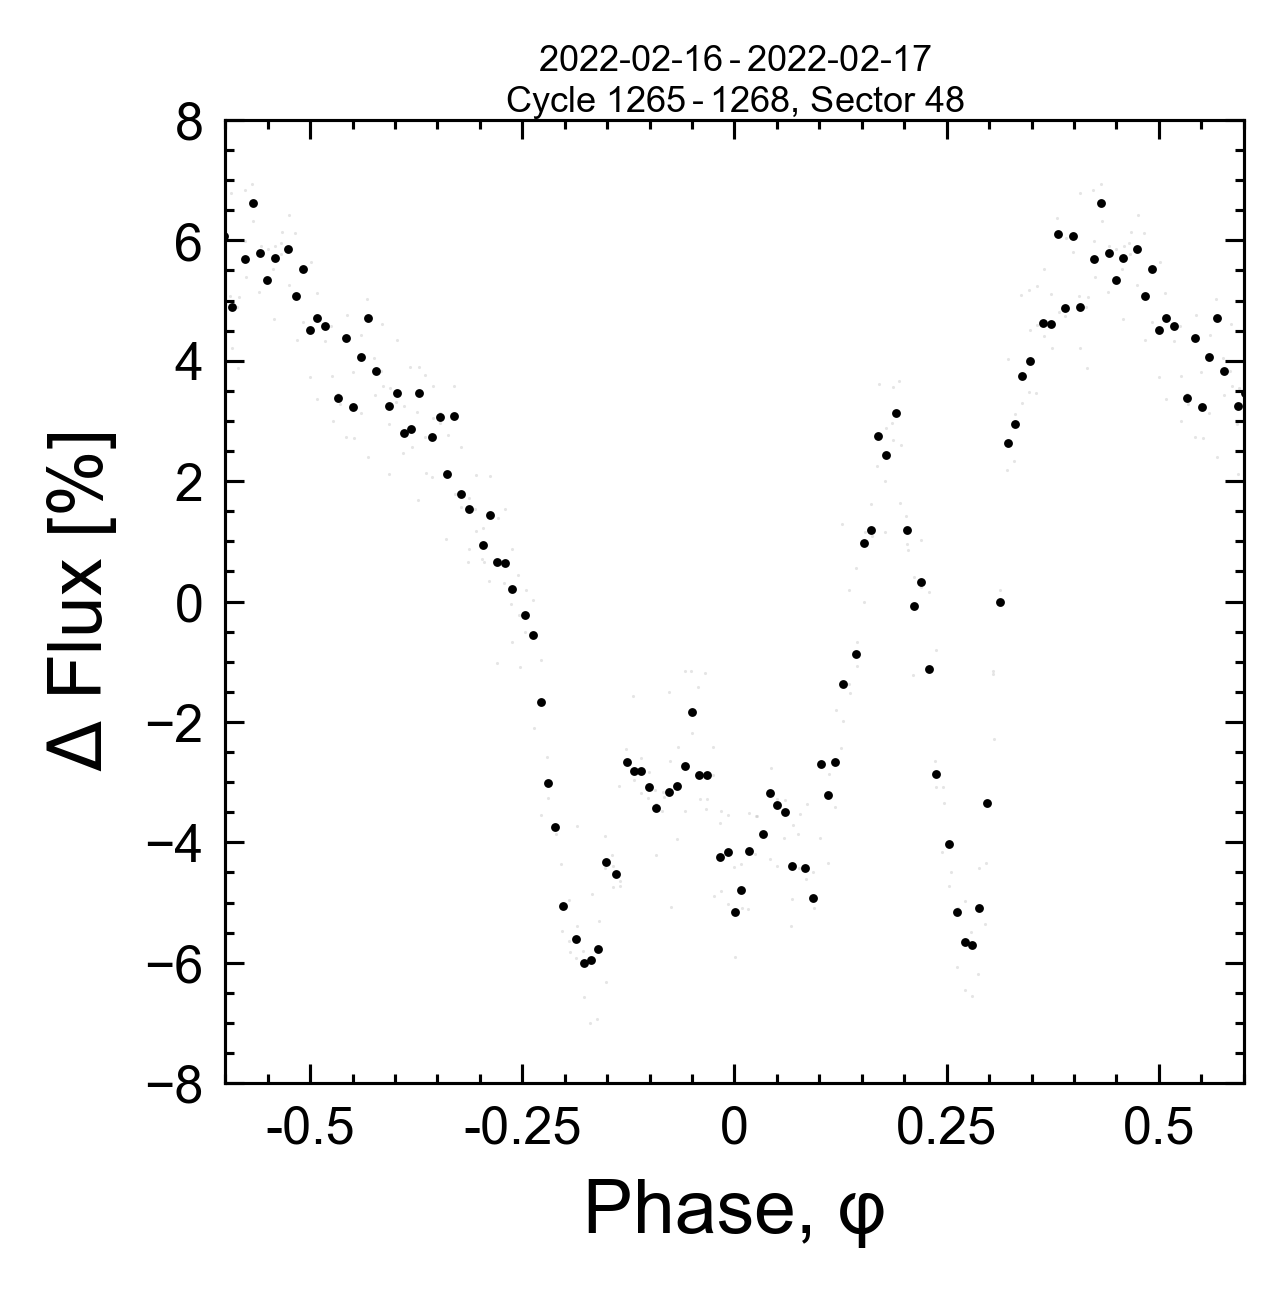
\includegraphics[width=0.7\textwidth]{figures/f1.png}
  \caption[]{{\bf Figure 1 (Movie):  TIC~141146667 is a complex periodic
  variable (CPV).} For the best experience, please view the online movie
  available
  \href{https://lgbouma.com/movies/movie_TIC1411_flux_phase.mp4}{here},
  which spans a baseline of 5{,}784 cycles irregularly sampled over three
  years.  The TESS light curve is phased to the \periodhr\ hour period in
  groups of a few cycles per frame.  This is the period both of
  stellar rotation, and (we hypothesize) of corotating clumps of
  circumstellar material.  Raw data acquired with two minute
  sampling are in gray; black is their average.  Similar to other members
  of this class, the sharp photometric features persist for tens to
  thousands of rotational cycles. }
  \label{fig:lc}
\end{figure}


The dearth of evidence for circumstellar material around CPVs is
surprising given that separate studies of young BAFGKM stars have, for
decades, reported that stellar coronae contain both hot ($10^6$ K) and
cool ($10^4$ K) plasma. In particular, time-series spectroscopy has
shown periodic high-velocity absorption and emission in Balmer lines
such as H$\alpha$, caused by long-lived, corotating clumps of cool
plasma \cite{CollierCameron1989,Donati2000,Dunstone2006,Skelly2008}.
Such clumps are forced into corotation by the magnetic field, and the
exact geometry of where the plasma can accumulate is dictated by the
magnetic field's topology.  For instance, a tilted dipole field tends
to yield an accumulation surface of a warped torus
\cite{Townsend2005}, whereas in the limit of a single strong field
line, accumulation occurs at the line's apex, furthest from the star
\cite{Waugh2022}.
However, none of these spectroscopic variables have shown any
photometric anomalies \cite{Bouma2024}, leaving open the issue of
whether they are related to CPVs.
A circumstantial argument that they might is that CPVs do respond to
sudden magnetic field changes: the otherwise long-lived eclipse
features often disappear following stellar flares
\cite{Stauffer2017,Bouma2024}.

In this study, we present the first observations of corotating clumps
of cool plasma around a CPV.  We identified TIC~141146667 in previous
work \cite{Bouma2024} by searching the TESS two-minute data for stars
showing periodic variability with at least three sharp dips per cycle.
We selected the star for spectroscopic observations because its
brightness and rapid rotation offered sensitivity to small variations
in the line profiles.  We observed it for five hours on UT 2024-02-17
using the High Resolution Echelle Spectrometer (HIRES;
\cite{vogt_hires_1994}) on the Keck I 10m telescope.  TESS observed
the star from UT 2024-02-05 to UT 2024-02-26 with a duty cycle of
XX\%.  TESS was finishing a data downlink during the spectral
observations, and photometric data collection resumed three rotation
cycles (12 hours) after the spectra were acquired.  Extended Data
Figure~\ref{fig:fulllc} shows the detailed photometric behavior of the
star before and after the exact epoch of observation; the star
remained sufficiently stable to not affect the interpretation that
follows.


\section{Results}

\begin{figure}[!tp]
  \centering
  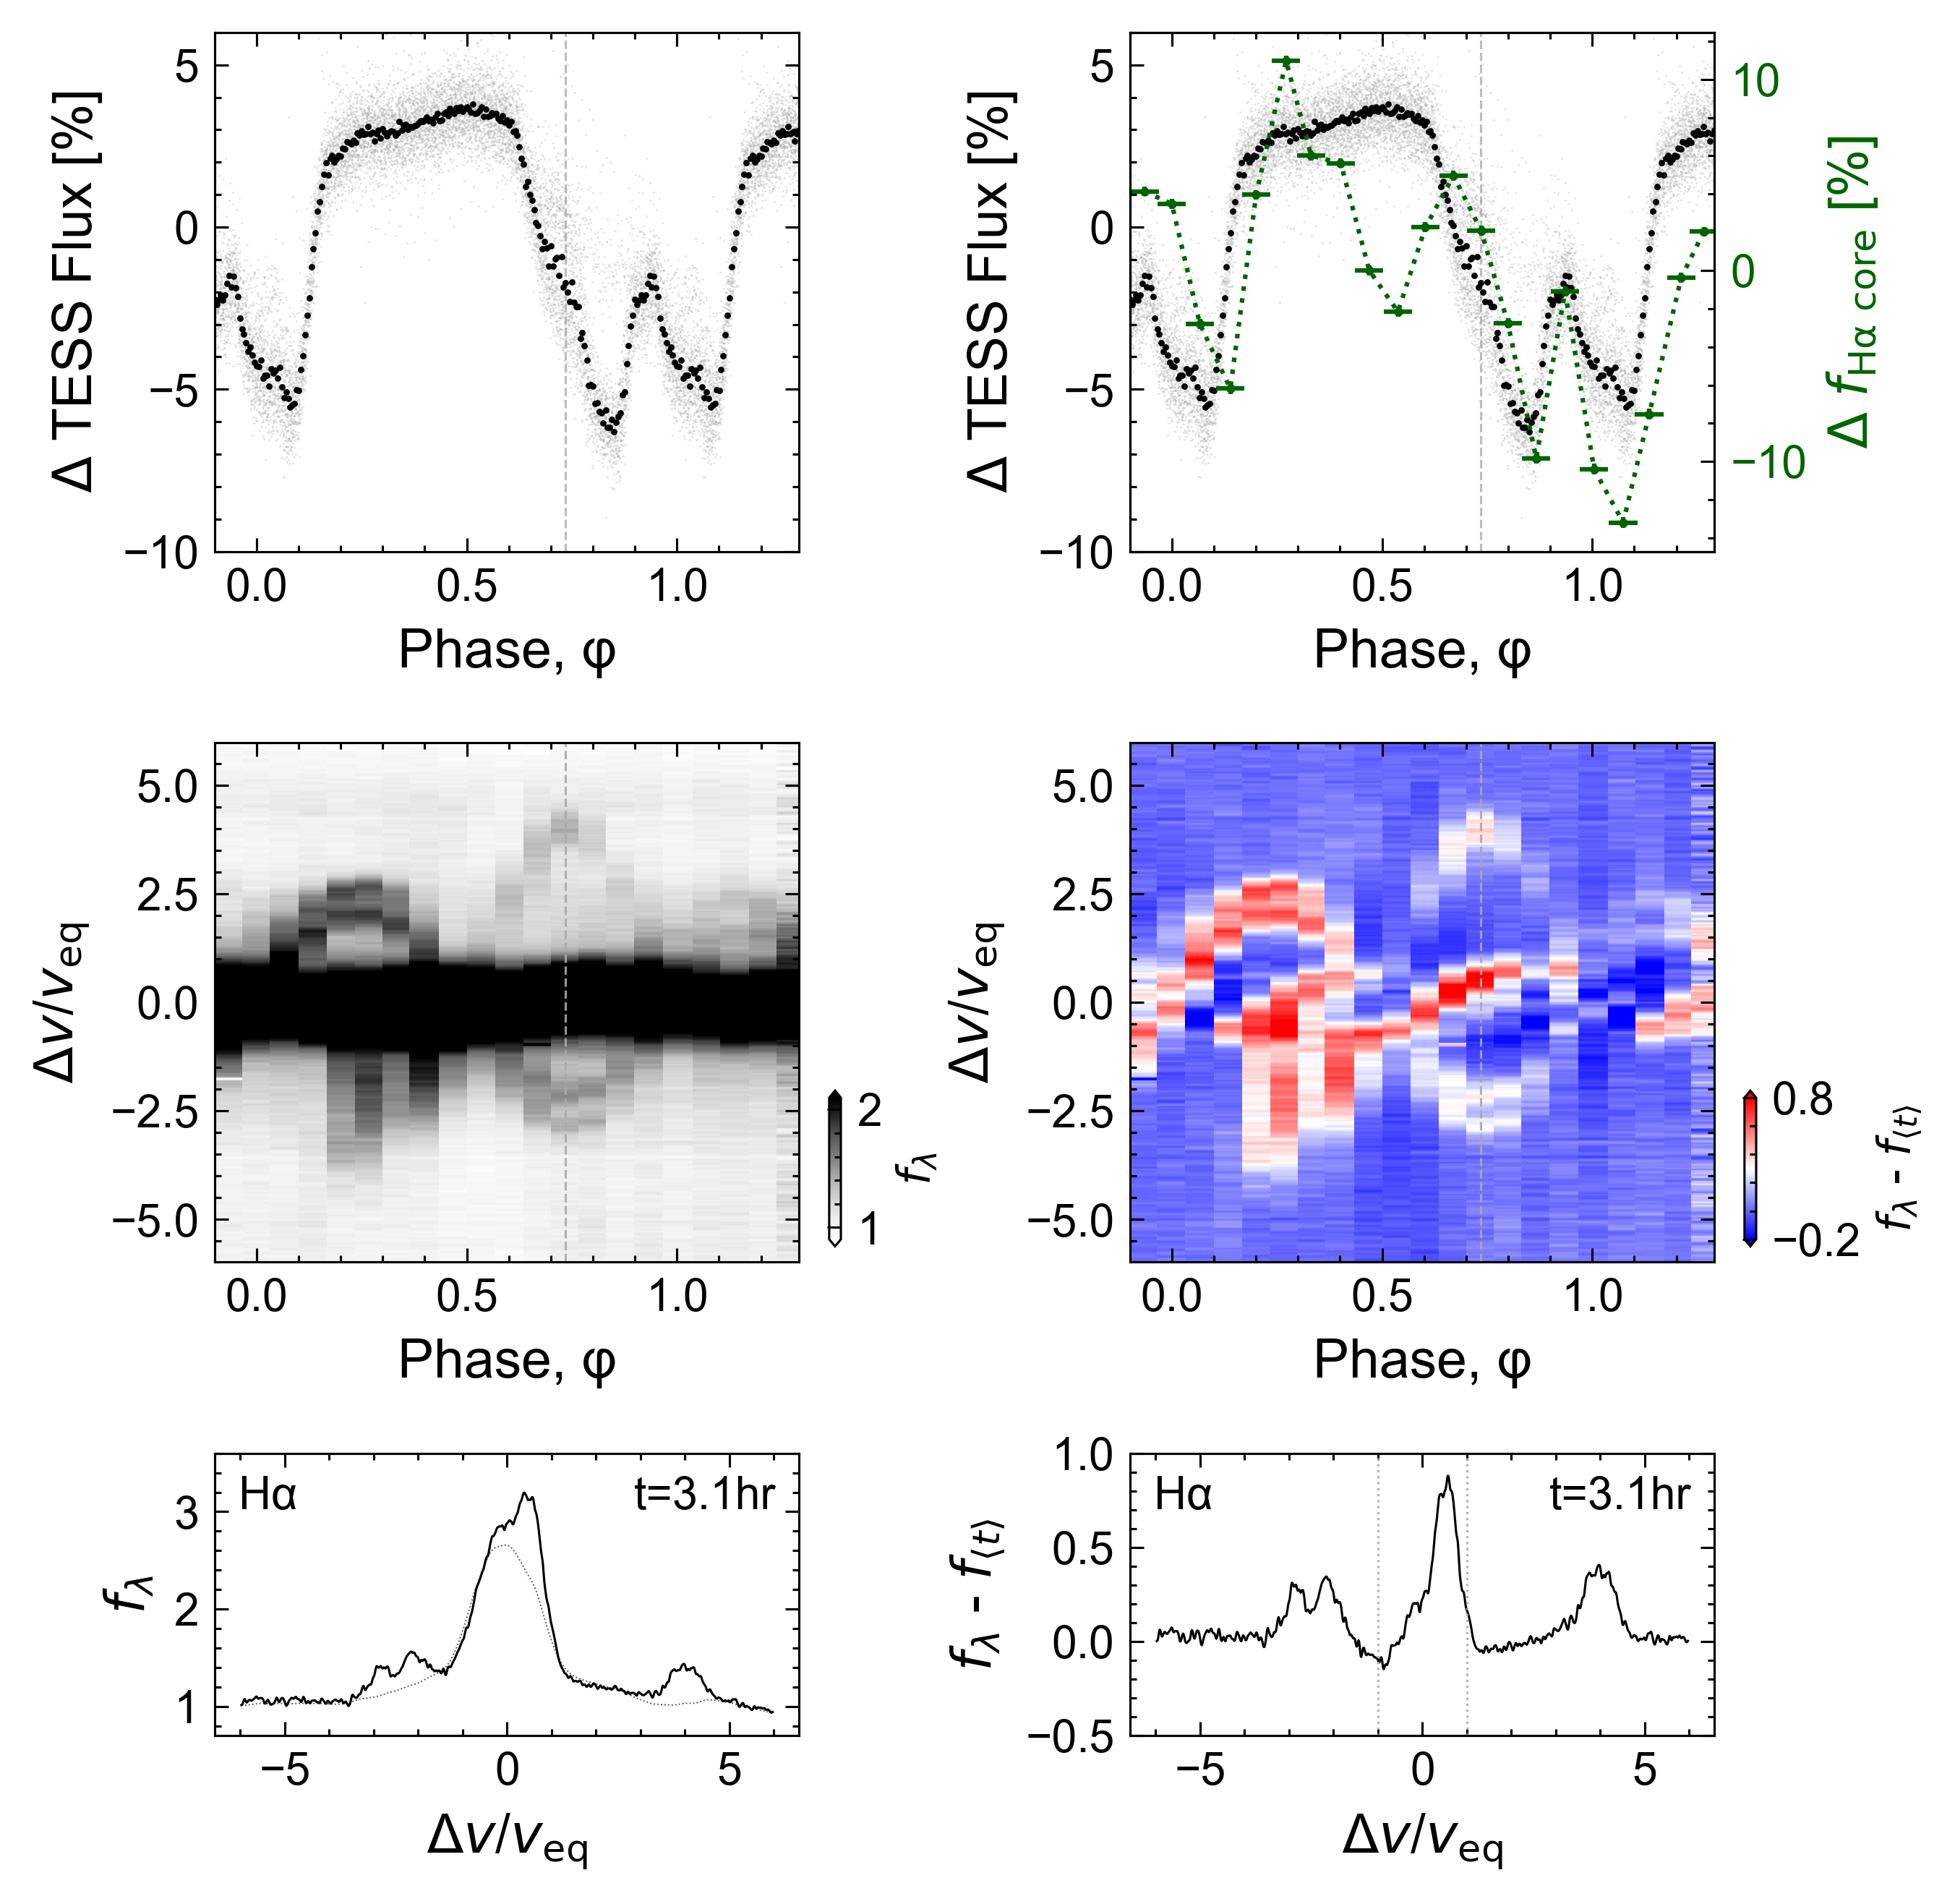
\includegraphics[width=0.99\textwidth]{figures/f2.png}
  \caption[]{{\bf Figure 2 (Movie):}  
  Hydrogen emission from circumstellar plasma orbiting TIC 141146667.
  {(\bf TODO)}For the best experience, please view the online movie
  available
  \href{https://lgbouma.com/movies/TIC141146667_sixpanel.mp4}{here}.
  {\bf Panel a:} TESS light curve from UT 2024-02-05 to UT
  2024-02-26 folded on the \periodhr\ hour period.  Black points are
  averaged; gray are the raw data.
  {\bf Panel b:} Keck/HIRES H$\alpha$ spectra
  acquired on UT 2024-02-17.  The continuum is set to unity, and the
  darkest color is set at twice the continuum to accentuate emission
  outside the line core ($|v/v_{\rm eq}|>1$, for $v_{\rm eq}$=130\,\kms).
  While emission in the line core originates in the stellar
  chromosphere, the sinusoidal emission features are most readily
  described by a warped plasma torus.
  {\bf Panel c:} Individual epochs of Panel b, visible in the
  online movie.  The dotted line shows a time-averaged spectrum,
  $f_{\langle t \rangle}$.
  {\bf Panel d:} As in Panel a, but overplotting the
  median-normalized H$\alpha$ light curve at $|v/v_{\rm eq}|<1$.
  {\bf Panel e:} As in Panel b, after subtracting the time-averaged
  spectrum. In addition to circumstellar emission, the line core shows
  absorption during the plasma clump transits.  The asymmetric stretch
  is set to match the dynamic range of the data.
  {\bf Panel f:} Individual epochs of Panel e, visible in the online
  movie.}
  \label{fig:spec}
\end{figure}

% photometry
Figure~\ref{fig:spec} shows the data from February 2024.  Similar to
other CPVs \cite{Bouma2024}, the photometric shape of
TIC~141146667 evolved following the 2022 discovery
data, while nonetheless remaining complex.  In February 2024, the
average photometric signal showed a gradual brightening over 45\% of
the period, followed by a complex eclipse-like feature spanning 55\%
of the period.  This eclipse feature shows two to three
local photometric minima, and one to two local maxima.
Its W-shape is suggestive of eclipse geometries seen in forward models
of warped plasma tori \cite{Townsend2008}.

% ** keck/hires: emission beyond v/veq>1
The spectroscopy shows emission well beyond the star's equatorial
velocity ($v_{\rm eq}$=130\,\kms).  There are at least two distinct
emission components, separated by half a cycle in phase.  The
first component has clearer sinusoidal behaviour and is double-peaked, with peak
semi-amplitudes of $K_1$=2.1\,$v_{\rm eq}$ and 2.7\,$v_{\rm eq}$.
There is significant non-periodic variability in this double-peaked
component: the flux excess from both peaks begins with an amplitude
equal to 100\% of the continuum flux early in the observation
sequence, and falls to 30\% by its end.  The component 180$^\circ$
opposite in phase is similarly only detected from $\phi$=0.2-1.0.
From $\phi$=0.2-0.5, this latter component appears connected to the
star in velocity space.  While its peak semi-amplitude of
$K_1$=3.9\,$v_{\rm eq}$ is achieved at both $\phi$=0.25 and 0.75, its
amplitude decreases from a 60\% excess over the continuum at the
beginning of the observation sequence to a 10\% excess by its end.
The sinusoidal period for all of these emission components is consistent
with the photometric \periodhr\ hour period.  

These sinusoidal emission features require circumstellar clumps of
partially-ionized hydrogen to be corotating with the star.  The
velocity semi-amplitude of the sinusoids gives the distance
of these clumps from the stellar surface: 2.1-2.7\,$R_\star$ for the
closer clump, and 3.9\,$R_\star$ for the other.  This material's
motion, rather than being Keplerian, can only be explained by plasma
being dragged along with the rotating stellar magnetic field.  These
clumps transit in front of the star when passing from negative to
positive velocity.

% * keck/hires: behavior at v/veq<1
The behavior within the stellar H$\alpha$ line core, at $|\Delta v /
v_{\rm eq}|<1$, is more complex than outside it.  For stars of
this age and spectral type, one would expect emission in the line core
to be generated in the stellar chromosphere
and then modulated by any occulting material capable of absorbing or
emitting H$\alpha$ photons.  In Figure~\ref{fig:spec}e, the behavior from
$\phi$=0.4-1.2 has a simple interpretation: from $\phi$=0.4-0.9, a hot
region first gradually crosses the stellar line profile, followed from
$\phi$=0.7-1.2 by the transit of a cool region.  Phases $\phi$$<$0.4
show a mix of similar events, though the time sampling is
sufficiently coarse that the interpretation is less clear.  A final
exercise to quantify the behavior in the line core is shown in
Figure~\ref{fig:spec}d, where $f_{\rm H\alpha\ core}$ denotes the
summed flux at $|\Delta v / v_{\rm eq}|<1$.  This panel shows that
changes in the line core flux are usually correlated with the
broadband variability, except at $\phi$=0.5, during the transit of the
higher-velocity clump and the occultation of the lower-velocity clump.

\begin{table*}
\scriptsize
\setlength{\tabcolsep}{2pt}
\centering
\caption{Selected System Parameters for TIC~141146667}
\label{tab:params}
\begin{tabular}{llcc}
\hline \hline
Parameter & Description & Value & Source\\
\hline 
%
$T_{\rm eff}$\dotfill                   & Effective Temperature (K) \hspace{9pt}\dotfill                 & 2972 $\pm$ 40    & 1 \\
%
%$\log{g_{\star}}$\dotfill              & Surface Gravity (cgs)\hspace{9pt}\dotfill                      & YYY              & X \\
%
$R_\star$\dotfill                       & Stellar radius ($R_\odot$)\dotfill                             & 0.42$\pm$0.02    & 1 \\
%
$M_\star$\dotfill                       & Stellar mass ($M_\odot$)\dotfill                               & XXX  & 6 \\
%
$\gamma$\dotfill                        & Systemic radial velocity (\kms)\dotfill                        & 0.61 $\pm$ 1.47  & 1  \\
%
Age                                     & Adopted stellar age (Myr)\dotfill                              & YYY  & 8 \\
%
Spec. Type\dotfill                      & Spectral Type\dotfill                                          & MXV              & X \\
%
$P_{\rm rot}$\dotfill                   & Rotation period (hr)\dotfill                                   & $3.930\pm 0.001$ & X \\
%
$v_{\rm eq}$\dotfill		                & Equatorial velocity \dotfill                                   &  130$\pm$4       & - \\
                                        & \hspace{3pt} ($2\pi R_\star/P_{\rm rot}$) (\kms)	             &                      \\
%
$v_{\rm eq}\sin{i_\star}$\dotfill		    & Projected rotational\dotfill                                   &  128$\pm$3       & X \\
                                        & \hspace{3pt} velocity (\kms)	                                 &                      \\
%
$i_\star$\dotfill                       & Stellar inclination (deg)\dotfill                              & 	XXX             & X \\
%
$d$\dotfill                             & Distance (pc)\dotfill                                          & $57.6 \pm X.X$   & X \\
%
$R_{\rm c}$\dotfill		                  & Keplerian corotation\dotfill                                   &  XXX             & X \\
                                        & \hspace{3pt} radius ($R_\star$)	                               &                      \\
%
$a_1$\dotfill                           & Clump 1 orbital radius ($R_\star$)\hspace{9pt}\dotfill         &  2.1-2.7         & X \\
$a_2$\dotfill                           & Clump 2 orbital radius ($R_\star$)\hspace{9pt}\dotfill         &  3.9             & X \\
%
$\langle$EW$_{\rm H\alpha}$$\rangle$    & Time-averaged H$\alpha$ line core                              &  X.X             & Y \\ 
                                        & \hspace{3pt} equivalent width (\AA)	                           &                      \\
Range(EW$_{\rm H\alpha}$)$_1$           & H$\alpha$ equiv. width range                                   &  X.X             & Y \\ 
                                        & \hspace{3pt} from Clump 1 (\AA)	                               &                      \\
Range(EW$_{\rm H\alpha}$)$_2$           & H$\alpha$ equiv. width range                                   &  X.X             & Y \\ 
                                        & \hspace{3pt} from Clump 2 (\AA)	                               &                      \\
\hline
\end{tabular}
\begin{flushleft}
\footnotesize{ \textsc{NOTE}---
%$^\dagger$ The GAIADR2 and GAIAEDR3 identifiers for Kepler 1627A are identical.  The secondary
is not resolved in the Gaia point source catalog.
$^*$ Given only $v\sin i$ and $2\pi R_\star/P_{\rm rot}$, $\cos i=0.11^{+0.11}_{-0.08}$.
Provenances are:
1: SED fit\cite{Bouma2024},
%$^6$Cluster isochrone (MIST adopted; PARSEC compared for quoted
%  uncertainty),
2: TESS light curve,
%  3: HIRES spectra and specmatch(?),
%$^8$Pre-main-sequence CAMD interpolation (Section~\ref{sec:camd}),
}
\end{flushleft}
\vspace{-0.5cm}
\end{table*}



\section{Discussion}
% argue: how does this clarify wider phenomenology?  what general
% conclusions can be drawn?

Spectra of magetically-active, rapidly rotating stars with a wide range of masses
have been known to exhibit both sinusoidal emission features
\cite{Donati2000,Townsend2005,Dunstone2006,Skelly2008} as well as
sharp transient absorption features in their line cores
\cite{CollierCameron1989,CollierCameron1992,Cang2020} similar to 
Figure~\ref{fig:spec}.  No such stars were previously known to show
complex light curves \cite{Bouma2024}.  The usual interpretation for
such variability comes from a loose analogy to
quiescent solar prominences, which are cool
condensations of plasma in the solar corona that can last days to
weeks \cite{VialEngvold2015}.
In our Sun's
magnetosphere, these condensations fall back to the solar surface
because gravity is stronger than any magnetic or centrifugal force
capable of sustaining them.  However for stars with magnetospheric
radii $R_{\rm m}$ that exceed their corotation radii $R_{\rm c}$, the
effective potential experienced by a plasma parcel can have a local minimum
outside $R_{\rm c}$, enabling the material to be sustained for
much longer timescales \cite{Petit2013,Daley-Yates2024}.  Generally
speaking, such material need neither transit, nor be optically thick.

Our Keck/HIRES observations are the first reported time-series
spectra of a CPV, and they show that corotating circumstellar plasma clumps 
are present in at least one such star.
Characteristic densities and masses of these
clumps are $n \sim 10^{10}$\,cm$^{-3}$ and $M \sim 10^{14}$\,kg (see
Supplementary Methods Section~\ref{subsec:model}), a similar density
to solar prominences, but ten to one hundred times more massive.  This
observation rules out a ``starspot-only'' origin scenario for CPVs,
\cite{Koen2021} since such scenarios have no means of explaining
spectroscopic emission beyond the stellar disk.  Similarly, scenarios
in which the circumstellar material is made only of dust are also
ruled out.  While dust may be present, to explain the H$\alpha$
emission the circumstellar clumps must include plasma with a
significant population of hydrogen atoms in the $n$=3 excited state.
While this plasma is undoubtedly sculpted by the star's magnetic
field, it could plausibly originate from three sites: the star, an old
and undetected disk, or outgassing rocky bodies.  This latter
possibility would render CPVs as extrasolar analogs of the Jupiter-Io
plasma torus (CITE).

The other potential analog for the CPVs are the $\sigma$~Ori~E
variables, a rare subset of B stars that with radiatively-driven winds
that can accumulate into
warped plasma tori \cite{Townsend2005,Townsend2008}.  These tori tend
to have dense antipodal accumulations of plasma sculpted by
tilted-dipole magnetic fields, and the transits of
these clumps are thought to produce the observed broadband photometric variability
through bound-free scattering \cite{Townsend2005} and
Thomson scattering \cite{Berry2022}.  For $\sigma$~Ori~E and almost
all of its analogs, the result is light curves that appear ``simple'',
resembling those of eclipsing binaries \cite{Townsend2008}.  The two known
exceptions, HD~37776 and HD~64740, show complex light curves
resembling CPVs \cite{Mikulasek2020,Bouma2024} and have
spectropolarimetric magnetic field maps indicating strong
contributions from higher-order magnetic moments
\cite{Kochukhov2011,Shultz2018}.  There are two implications: first,
the complexity of CPVs may be a direct consequence of magnetic fields
with highly multipolar contributions.  Second, CPVs could be a
source of astrophysical false positives in photometric searches for
eclipsing binaries and transiting exoplanets around young
pre-main-sequence M dwarfs \cite{Johns-Krull2016,Bouma2020}.

Pressing issues for future work include determining the composition
and origin of the circumstellar material, understanding the exact role
of the stellar magnetic field, and exploring the implied space weather
experienced by the close-in rocky exoplanets that, statistically
\cite{Dressing2015}, are likely to be present in most CPV systems.

The material's composition -- either pure plasma, or else a dusty
plasma -- can be clarified by time-series optical and infrared
spectrophotometry.  While observations of CPVs in the optical have
previously suggested chromaticity consistent with dust \cite{Tanimoto2020,Gunther2022,Koen2023},
a gray opacity source such as electron scattering in a plasma
transiting over starspots could also produce chromatic features
\cite{Rackham2018}.  The composition and size distribution of any dust
that is present could be most easily resolved by measuring the
extinction curve for one or more CPVs from 1-10\,$\mu$m.  A
dust composition similar to debris from rocky bodies seen around white
dwarfs \cite{Reach2009} would indicate a rocky-body origin.  A 
composition closer to the ISM would be indicative of condensed dust in
an M dwarf wind, similar to that formed in the environments of more
evolved stars \cite{Marigo2008}.

The role of the star's magnetic field could be better understood
through new observations, and new theory.  From the theoretical
perspective, there is an urgent need for rigid-field
(magneto)-hydrodynamic modeling to go beyond previous work
\cite{Townsend2005,Townsend2008} and to explore the effects of
non-dipolar field contributions.
In particular, dynamo simulations of fully-convective M dwarfs have
suggested the possibility that global-scale mean fields can be
confined to a single hemisphere \cite{Brown2020}; such fields would
yield accumulations of circumstellar material quite different
from those that have previously been explored \cite{Townsend2008}.
Observationally, spectropolarimetry has the potential to
assess both the field strength and topology.  An independent
probe could also be connected the recent work \cite{Kaur2024} showing
that CPVs are variable radio emitters with emission components
that can be both persistent, and also short-lived and highly
polarized.  In particular, detecting radio emission
from the electron cyclotron maser instability would
provide a direct measurement of the field strength at the site of the
emitting region.

It is currently unclear what, if any, relationship CPVs have to the
close-in exoplanets that exist around most M dwarfs
\cite{Dressing2015}.  However, 0.3-3\% of young M dwarfs show the CPV
phenomenon \cite{Rebull2020}, and our data show that the phenomenon
occurs when clumps of circumstellar material transit the star.  The
implied geometric correction suggests that an appreciable minority
(3-30\%) of M dwarfs -- the rapidly rotating ones with centrifugal
magnetospheres -- have similar circumstellar environments to the CPVs.




%%%%%%%%%%%%%%%%%%%%%%%%%%%%%%%%%%%%%%%%%%%%%%%%%%%%%%%%%%%%%%%%%%%%%%%%%%%%%%%
%%%%%%%%%%%%%%%%%%%%%%%%%%%%%%%%%%%%%%%%%%%%%%%%%%%%%%%%%%%%%%%%%%%%%%%%%%%%%%%

\newpage
\begin{methods}

\renewcommand{\figurename}{Extended Data Figure}
\renewcommand{\tablename}{Extended Data Table}
\setcounter{table}{0}  
\setcounter{figure}{0}  

\subsection{Observations \& Data Reduction}\phantom{+}

\begin{figure}[!b]
  \centering
  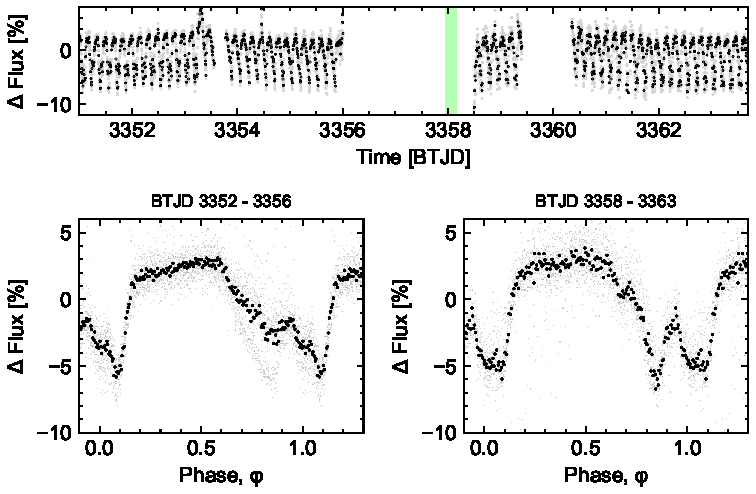
\includegraphics[width=0.99\textwidth]{figures/sf1.pdf}
  \caption{Photometric evolution of TIC 141146667 near the epoch of
  spectroscopic observation (green bar). 
  {\bf Panel a}: TESS simple aperture photometry. 
  The main data gaps were caused by scattered light from the Earth
  (BTJD 3356-3358.5) and Moon (BTJD 3359.5-3360.5).
  {\bf Panels b,c}: Folded light curve before and after spectroscopy.
  While some evolution in the light curve morphology occurred between
  the two epochs, the large, complex eclipse feature remained present.
  }
  \label{fig:fulllc}
\end{figure}

{\it Photometry:} TESS observed
TIC~141146667 ($T$=13.3) in Sectors 14, 15, 21, 41, 48, and 75.
Two-minute data were acquired during Sectors 41, 48 (TESS DDT039,
PI: Kunimoto), and 75 (TESS Program G06030, PI: Bouma).  The data
from Sectors 14, 15, and 21 had a 30-minute cadence, which
smears sharp features over the $<$4\,hour period
(see \cite{Gunther2022}).  The nearest known star, TIC~141146666
($T$=14.5), is 25$''$ from TIC~141146667 and is photometrically stable
in the pixel-level TESS data.

Figure~\ref{fig:fulllc} shows the data from Sector~75, which were
acquired using the camera that points closest to the ecliptic.  The
largest gap in coverage is from BTJD 3356.0~-~3358.5, and includes
the Keck/HIRES observation epoch (green bar).   There are no flux
measurements reported during this interval because the Earth was
within 25$^\circ$ the camera's boresight, yielding high levels of
scattered light.  From BTJD 3359.4~-~3362.0, the Moon then passed
within 25$^\circ$ of the camera's boresight.  Based on the observed
level of scattered light in the optimal TIC~141146667 aperture, we
manually masked out times from 3359.4~-~3360.13, and judged the
remainder of the data during the lunar approach to be usable.  The
small data gaps from BTJD 3353.55~-~3353.77 and from BTJD
3360.12~-~3360.33 were caused by data downlinks at the spacecraft's
perigee and apogee, respectively.

{\it Spectroscopy:}
We observed TIC~141146667 ($V$=16.2) with Keck/HIRES for five hours over a
second-half night spanning UT 2024-02-17 10:47 to UT 2024-02-17
16:13.  The star's airmass over this window spanned $z$=1.2-2.2, and
we opted for a fixed 15 minute cadence over the entire sequence,
except for a final 10 minute exposure due to increasing sky
brightness at sunrise.  We observed without the iodine cell and used
the C2 decker (0$\farcs$86$\times$14$\farcs$0) in the red instrument
configuration, yielding a spectral resolution $R$$\approx$45{,}0000
($\delta v$$\approx$6.7\,\kms; $\delta v / v_{\rm
eq}$$\approx$0.05).  We binned the CCD readout by a factor of three
in the spatial dimension, yielding $\approx$1,000 photons (S/N=33)
per pixel in the continuum at 6500\,\AA, at minimum airmass.  Strong
winds contributed to 1\farcs2$\pm$0\farcs2 seeing over the night,
but conditions were otherwise favorable.  We reduced the
echelleogram to a one-dimensional spectrum using the standard
techniques of the California Planet Survey \cite{Howard2010}.
Figure~\ref{fig:spec} shows the result in the vicinity of H$\alpha$
without any additional processing.


\subsection{Stellar Parameters}\phantom{+}

{\it Radial Velocity}---We measured radial velocities of
TIC~141146667 from each of our spectra using a pipeline that we
developed specifically for rapidly rotating stars.
Our method is based on template-matching against synthetic spectra
produced by the PHOENIX stellar atmosphere code \cite{Husser2013}.
We used the PHOENIX models with solar metallicity and alpha element
abundances, and calibrated our absolute velocity zero-points as well
as viable orders for velocity measurement using the
standard stars described by \cite{Chubak2012}.
We used velocity standards spanning spectral types from G2 to M4 (Barnard's
Star), irrespective of rotation rate.
We used \texttt{barycorrpy} \cite{Kanodia2018} to calculate the
velocity corrections due to Earth's motion around the solar system
barycenter and due to Earth's daily rotation about its axis.
Our analysis pipeline reproduces the systemic velocities reported by
\cite{Chubak2012} for their velocity standards with an RMS of
0.66\,\kms.

For TIC~141146667, we measured the velocities from each of our HIRES
spectra using regions near the K~I (7700\,\AA) resonance line and
three TiO bandheads (5160\,\AA, 5450\,\AA, and 5600\,\AA).  These
regions were selected because they provided the best matches between
the synthetic and observed spectra.  The resulting redshift
measurements were averaged together.  The star's 130$\pm$4\,\kms\
equatorial velocity and near-edge on viewing orientation yielded a
line broadening $\Delta \lambda$$\approx$3\,\AA.  We used the scatter
of resulting velocity measurements between orders to assign the RV
uncertainty at each epoch.  The uncertainty-weighted mean systemic
velocity over all epochs on UT 2024-02-17 was
$\gamma$=0.6$\pm$1.5\,\kms.  The relative radial velocities about this
mean are given in Table~\ref{tab:rv}.
% from calc_max_amplitude_sinusoid_rv_timeseries.py
% from K_to_msini.py, assuming Mstar = 0.18

{\it No Evidence For Binarity}---Any significant periodicity in the
radial velocity time-series is ruled out at the rotation period for
semi-amplitudes above 2.85\,\kms\ (at 3$\sigma$ confidence).  This
sets an upper limit on the mass of any putative companions at the four
hour period of $m \sin i $$<$2.4\,$M_{\rm Jup}$.  Regarding possible
companions at wider separations, the Gaia DR3 renormalized unit weight
error (RUWE), a proxy for the goodness of fit for a single-source
astrometric model to the Gaia astrometry, is 1.23, which is within the
usual range for apparently single sources.  There are no resolved
sources in the Gaia DR3 point source catalog.  Finally, we checked the
TESS light curve for evidence of secondary photometric periods by
subtracting the mean CPV signal over each sector and performing a
phase-dispersion minimization analysis
\cite{Stellingwerf1978,2021zndo...1011188B}.  There were no secondary
periods in the TESS data.  Previous work \cite{Bouma2024} has shown
that about 30\% of CPVs show evidence for excess noise above the Gaia
single-source astrometric model, and about 40\% of CPVs show evidence
for unresolved binary companions based on the presence of secondary
photometric periods.  This agrees with analyses showing that
multi-periodic low-mass stars are generally unresolved binaries
\cite{Tokovinin2018}.  Overall, the CPV binary fraction seems
consistent with that for field M dwarfs \cite{Winters2019},
pointing to a weak or non-existent connection between the CPV
phenomenon and binarity.  For TIC~141146667 specifically, we find 
no evidence for stellar multiplicity.


{\it Age: No Obvious Association Membership}---Previous work
\cite{Bouma2024} has found that over 90\% of CPVs are associated with
known young moving groups based on their positions and kinematics.
TIC~141146667 is one of the exceptions.  We calculated the probability
of TIC~141146667 being part of any of the nearby known groups using
BANYAN\,$\Sigma$ v1.2 \cite{Gagne2018}.  Based on that model,
it appears to be a field star at $>$99.9\% confidence.  We also searched the
local vicinity of TIC~141146667 for neighbors with similar projected on-sky
velocities using \texttt{comove} \cite{Tofflemire2021}.  This yielded
no strong candidates for co-moving stars --- defined as those with
projected tangential velocities $\Delta v_{\rm T}$$<$5\,\kms ---
that share its isochronal youth.

{\it Age: Isochrones}---The color and absolute magnitude of
TIC~141146667 suggest that it is a pre-main-sequence M dwarf, similar
to all other known CPVs \cite{Stauffer2017,Stauffer2021,Bouma2024}.
The star's proximity ($d$=58\,pc) and its high galactic latitude
($b$=$+$53$^\circ$) yield negligible interstellar reddening along the
line of sight \cite{Green2019}.
{\bf Figure~X} shows the location of the star in the color--absolute
magnitude diagram (CAMD)
relative to young stellar populations including Upper Scorpius (USco),
Upper-Centaurus-Lupus (UCL), IC~2602, and the Pleiades.
To make this diagram, {\bf TODO}we adopted the USco and UCL members
from X, the IC~2602 members from Y, and the Pleiades members from Z,
and applied the same reddening corrections as in \cite{Bouma2022}.
To measure the isochrone age of TIC~141146667, we then followed the 
empirical approach proposed by \cite{Gagne2020} and
implemented in \cite{Bouma2022}.
The idea is to estimate the star (or star cluster's) age by
interpolating between the observed isochrones of star clusters with
ages that have been otherwise calibrated, for instance using
the lithium depletion-boundary method.
While this circumvents known modelling issues in molecular opacities
and starspot coverage for young M dwarfs,
the ages returned by this procedure depend on the ages
assumed for each reference cluster.
In this case, the most important reference is UCL, since TIC~141146667
overlaps directly on its isochrone on the CAMD.
We adopted the 16~Myr age for UCL from \cite{PecautMamajek2016}, which
is consistent with ages determined by more recent sub-clustering
analyses \cite{Ratzenbock2023} for the largest sub-populations.
This in turns yields an isochronal age for TIC~141146667 of
$t_{\rm iso}$=$16^{+19}_{-6}$\,Myr.
Qualitatively, this range of uncertainty is consistent with no stars
in the $\approx$40\,Myr IC~2602 cluster with similar redness as
TIC~141146667 being equally bright.

{\it Age: Lithium}--- Frankly, it's not obviously there!  (but maybe
this is bc of the blending, and a pEW would show smth small)
%TODO TODO TODO

% We have K=10.47, d=57pc - > DM ~= 3.78 -> M_K ~= 6.67
Figure7 of Wood23 suggests from the Feiden Li depletion curves that no lithium would imply $t$>37Myr.
However Figure5 frmo the same work suggests maybe try binning up the spectrum, and then comparing against Bochanski+2007 for a lithium-free template.

Try differential comparison against Barnard's star...

{\it Age: Summary}---The main indicators for the youth of
TIC~141146667 are {\it i)} that it is a complex periodic variable;
{\it ii)} that it is 1.5 magnitudes brighter than main sequence stars
of the same color, while showing no indicators for binarity; {\it
iii)} weak lithium absorption.





{\it Effective temperature, radius, and mass}
We adopt the results from the spectral energy distribution fitting
exercise described by \cite{Bouma2024}.
In brief, this approach used
\texttt{astroARIADNE}...
\cite{Vines2022} with the BT-Settl stellar
atmosphere models \cite{Allard2012} assuming the
\cite{Asplund2009} solar abundances, and the
\cite{Barber2006} water line lists.  
We used broadband magnitudes from Gaia DR2, APASS, 2MASS, SDSS, and WISE
  $W1$ and $W2$.  (explain)...

%%%%%%%%
%\texttt{astroARIADNE} compares the measured broadband flux
%measurements against pre-computed model grids, and by default fits for
%six parameters: $\{ T_{\rm eff}, R_\star, A_{\rm V}, \log g, [{\rm
%Fe/H}], d \}$.  The distance  prior is drawn from
%\citet{2021AJ....161..147B}.  The surface gravity and metallicity are
%generally unconstrained.  Given our selection criteria for the stars,
%we assumed the following priors for the temperature, stellar size, and
%extinction:
%\begin{align}
%  T_{\rm eff} / {\rm K}    &\sim \mathcal{U}(2000, 8000), \\
%  R_\star / R_\odot  &\sim \mathcal{U}(0.1, 1.5), \\
%  A_{\rm V} / {\rm mag}    &\sim \mathcal{U}(0, 0.2),
%\end{align}
%for \deleted{$\mathcal{N}$ the Gaussian and }$\mathcal{U}$ the uniform
%distribution\deleted{s, and $\mathcal{T}_{\rm N}(\mu, \sigma, a, b)$ a
%truncated normal distribution with mean $\mu$, standard deviation
%$\sigma$, and lower and upper bounds $a$ and $b$}.  We validated our
%chosen upper bound on $A_{\rm V}$ using a 2MASS color-color diagram.
%Finally, using \texttt{Dynesty} \citep{2020MNRAS.493.3132S}, we
%sampled the posterior probability assuming the default Gaussian
%likelihood, and set a stopping threshold of ${\rm d}\log \mathcal{Z} <
%0.01$, where $\mathcal{Z}$ denotes the evidence.


{\it SED: No evidence for disk}
...



\subsection{Spectroscopic Variability}\phantom{+}

The full HIRES coverage spans 3650-7960\,\AA, and variable
  emission is visible in Balmer lines from $n$=10$\rightarrow$2, Ca[H]
  and Ca[K], the Mg[I] b triplet, and the 5875 He[I] emission line.

%TODO: add figure showing spectral variability!



\subsection{Spectral Behavior of Other Lines}

First, chromospheric:

{\it H$\gamma$, H$\delta$}
Line ratios.

{\it Ca [K]}
{\it Also} shows some high-velocity emission.  So, the emitting material has
calcium ions.

{\it He 5880}
Also variable...

{\it Magnesium b orders}
Shows some variability that is horrendously blended.

{\it K[I] 7700}
Literally the only obvious photospheric line.



\subsection{Modeling the Emitting Clump}
\label{subsec:model}

% * mass estimate
The density and mass of the material...


%%%%%%%%%%%%%%%%%%%%%%%%%
% Supplementary Figures %
%%%%%%%%%%%%%%%%%%%%%%%%%

%%%%%%%%%%%%%%%%%%%%%%%%
% Supplementary Tables %
%%%%%%%%%%%%%%%%%%%%%%%%

% TEMPLATE: IRAS041
%
\begin{table}
    \centering
    \begin{tabular}{lcr}
    \hline 
    \hline
    Parameter & Host & Source \\
    \hline 
    \multicolumn{3}{c}{Identifiers} \\
    \hline
    TIC & 141146667 & TESS \\
    Gaia & 860453786736413568 & Gaia\ DR3 \\
    %2MASS & J04154278+2909597 & J04154269+2909558 & 2MASS \\
    %ALLWISE & J041542.77+290959.5 & ... & ALLWISE\\
    \hline
    \multicolumn{3}{c}{Astrometry} \\ 
    \hline
    $\alpha$ & todo & Gaia\ DR3 \\
    $\delta$ & todo & Gaia\ DR3 \\
    $\mu_{\alpha}$ (mas yr$^{-1}$ ) & -73.933 $\pm$ 0.022 & Gaia\ DR3 \\
    $\mu_{\delta}$ (mas yr$^{-1}$ ) &  32.262 $\pm$ 0.024 & Gaia\ DR3 \\
    $\pi$ (mas)                     &  17.324 $\pm$ 0.025 & Gaia\ DR3 \\
    RUWE                            &  1.23               & Gaia\ DR3 \\
    \hline
    \multicolumn{3}{c}{Photometry} \\
    \hline
    $TESS$ (mag) & todo & TESS\ \\
    $G$ (mag)                       & 14.701 $\pm$ 0.002 & Gaia\ DR3 \\
    $G_{\rm BP}$ (mag)              & 16.664 $\pm$ 0.008 & Gaia\ DR3 \\
    $G_{\rm RP}$ (mag)              & 13.398 $\pm$ 0.006 & Gaia\ DR3 \\
    $G_{\rm BP}$-$G_{\rm RP}$ (mag) &  3.276 $\pm$ 0.010 & Gaia\ DR3 \\
    $J$ (mag)                       & 11.401 $\pm$ 0.022 & 2MASS     \\
    $H$ (mag)                       & 10.793 $\pm$ 0.021 & 2MASS     \\
    $K_s$ (mag)                     & 10.473 $\pm$ 0.016 & 2MASS     \\
    $W1$ (mag)                      & 10.276 $\pm$ 0.023 & ALLWISE   \\ % Cutri+2013 II/328/allwise
    $W2$ (mag)                      & 10.070 $\pm$ 0.020 & ALLWISE   \\
    $W3$ (mag)                      &  9.838 $\pm$ 0.045 & ALLWISE   \\
    %$W4$ (mag)                      &  8.392 $\pm$ NOUNC & ALLWISE \\
	  %
    %TODO: eROSITA?  ROSAT is an emitter.  GALEX detection.
    % Ofek+2011 1.4Ghz emitter.  Helfand+2015 ditto.  Bruzewski+2021.
    \hline
    \multicolumn{3}{c}{Kinematics and Position} \\
    \hline
    $RV_{Bary}$ (km s$^{-1}$ ) & $13.35 \pm 3.39$ & HIRES \\
    $U$ (\kms) & & \\
    $V$ (\kms) & & \\
    $W$ (\kms) & & \\
    $X$ (pc) & -28.4 & \\
    $Y$ (pc) &  19.8 & \\
    $Z$ (pc) &  67.0 & \\
    \hline
    \multicolumn{3}{c}{Physical Properties} \\
    \hline
    $P_{rot}$ (hours) & $3.930 \pm 0.XXX$ & This work \\ 
    $v \sin i_\star$(km s$^{-1}$) & todo & This work\\
    $i_\star$($^\circ$) & todo & This work \\
    $T_{eff}$ (K) & 2972 $\pm$ 40 & \cite{Bouma2024}\\
    %$\log{g_{\star}}$\dotfill              & Surface Gravity (cgs)\hspace{9pt}\dotfill                      & YYY              & X \\
    $R_\star$ ($R_{\odot}$) & 0.42 $\pm$ 0.02 & \cite{Bouma2024} \\
    $A_V$ (mag) & 0 & \cite{Green2019} \\
    $F_{bol}$ (erg cm$^{-2}$ s$^{-1}$ ) & todo & This work\\
    $L_\star$ ($L_{\odot}$)  & todo & This work\\
    $M_\star$ ($M_{\odot}$)  & todo & This work\\
    $t_{\rm iso}$ (Myr) & $16^{+19}_{-6}$ &  This work \\
    \hline
    \end{tabular}
    \caption{Properties of \starname.}
    \label{tab:stellarParameters}
\end{table}


\begin{table}
  \centering
  \begin{tabular}{lcr}
  %\setlength{\tabcolsep}{2pt}
  \hline 
  \hline 
  Time [JD$_{\rm UTC}$] & RV (\kms) & $\sigma_{\rm RV}$ (\kms) \\
  % from tables/tab_TIC141146667_rel_rv.tex
  \hline 
  60357.450329 & 1.72 & 5.86 \\
  60357.461255 & -5.41 & 2.37 \\
  60357.472181 & -1.21 & 2.64 \\
  60357.483109 & 2.83 & 2.87 \\
  60357.494030 & 6.52 & 7.53 \\
  60357.504949 & -3.0 & 1.44 \\
  60357.515873 & 0.01 & 1.21 \\
  60357.526794 & -0.38 & 7.03 \\
  60357.537717 & -3.92 & 2.71 \\
  60357.548639 & 7.92 & 6.75 \\
  60357.559566 & 4.94 & 8.84 \\
  60357.570487 & -3.26 & 3.06 \\
  60357.581408 & 0.83 & 1.34 \\
  60357.592330 & 1.4 & 8.24 \\
  60357.603251 & -8.05 & 3.94 \\
  60357.614172 & -3.26 & 3.07 \\
  60357.625095 & -3.84 & 7.55 \\
  60357.636019 & -1.6 & 2.26 \\
  60357.646940 & 0.82 & 2.91 \\
  60357.657861 & 3.53 & 3.95 \\
  60357.668781 & 5.2 & 12.14 \\
  \hline
  \end{tabular}
  \caption{TIC~141146667 radial velocities.}
  \label{tab:rv}
\end{table}



\end{methods}

\bibliography{cpvbib.bib} % common bib file
\bibliographystyle{naturemagfixed}   


\begin{addendum}

\item[Acknowledgments]
  % convos w/
  % M.~Jardine. (line core sum, explaining flux tubes)
  % A Weinberger (dissolving rocks)
  % L Hillenbrand (general?)
  % line profile analysis by B.~Tofflemire.
  % CPS group for reduction support.
  The author thanks X, Y, Z.
  L.G.B. was suported by...
	Acknowledge TESS...


%TC:ignore
%% Author Contribution
\item[Author Contributions] ...
%TC:endignore

\item[Data Availability] ...

\item[Competing Interests] The authors declare that they have no competing
financial interests.
 
\item[Correspondence] Correspondence and requests for materials should be
addressed to ...
 
\item[Code availability] We provide access to a GitHub repository including all
code created for the analysis of this project that is not already publicly
available.

\end{addendum}



\end{document}


